% Appendices
% This should include detailed and technical documentation such as table of results, diagrams, program source code, etc, which are essential parts of the project but not directly a part of the main discussion in the report.  All contents of appendices should be exclusively, products of the student's own work.
% Other materials used during the project work (such as information from user manuals, interview notes, etc), which it is necessary to include, should if possible be summarized to only a few pages before entering into the appendix. Original copies of such material should be kept by the student and may be required to be produced as supporting evidence of their work.  Examples of key coding may be provided in an Appendix but generally it should be on the P drive with its associated software.
\subsection{Appendices}
% TODO: Discuss the debugging research process here?
\begin{figure}
    \centering
    \caption{Project Timeline}
    \label{fig:ProjectTimeline}
    \begin{subfigure}[t]{0.5\textwidth}
        \caption{Timeline table}
        \label{fig:ProjectTimelineChart}
        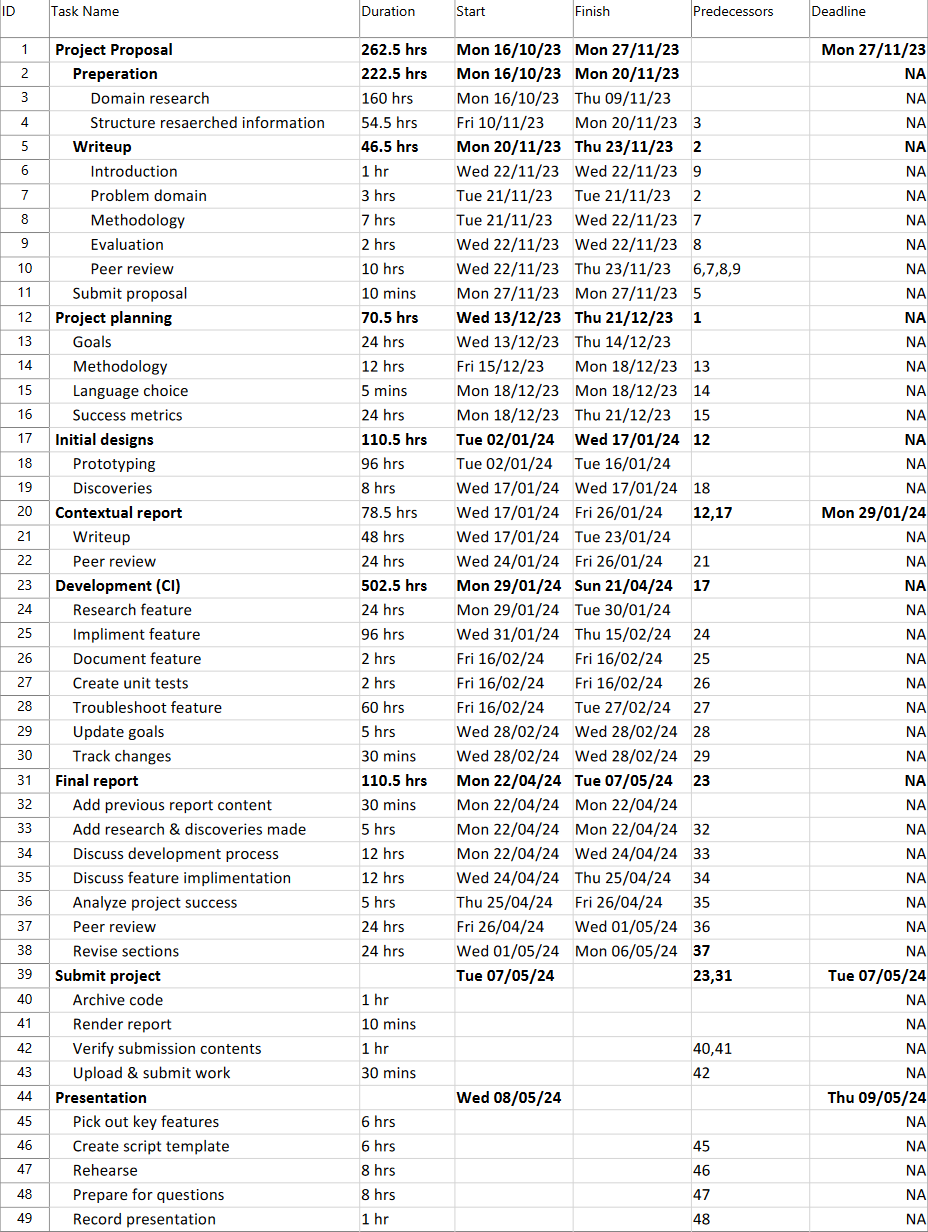
\includegraphics[clip, width=0.5\textheight]{../TimelineChart.png}
    \end{subfigure}
    \begin{subfigure}[b]{0.5\textwidth}
        \caption{Gantt chart}
        \label{fig:GanttChart}
        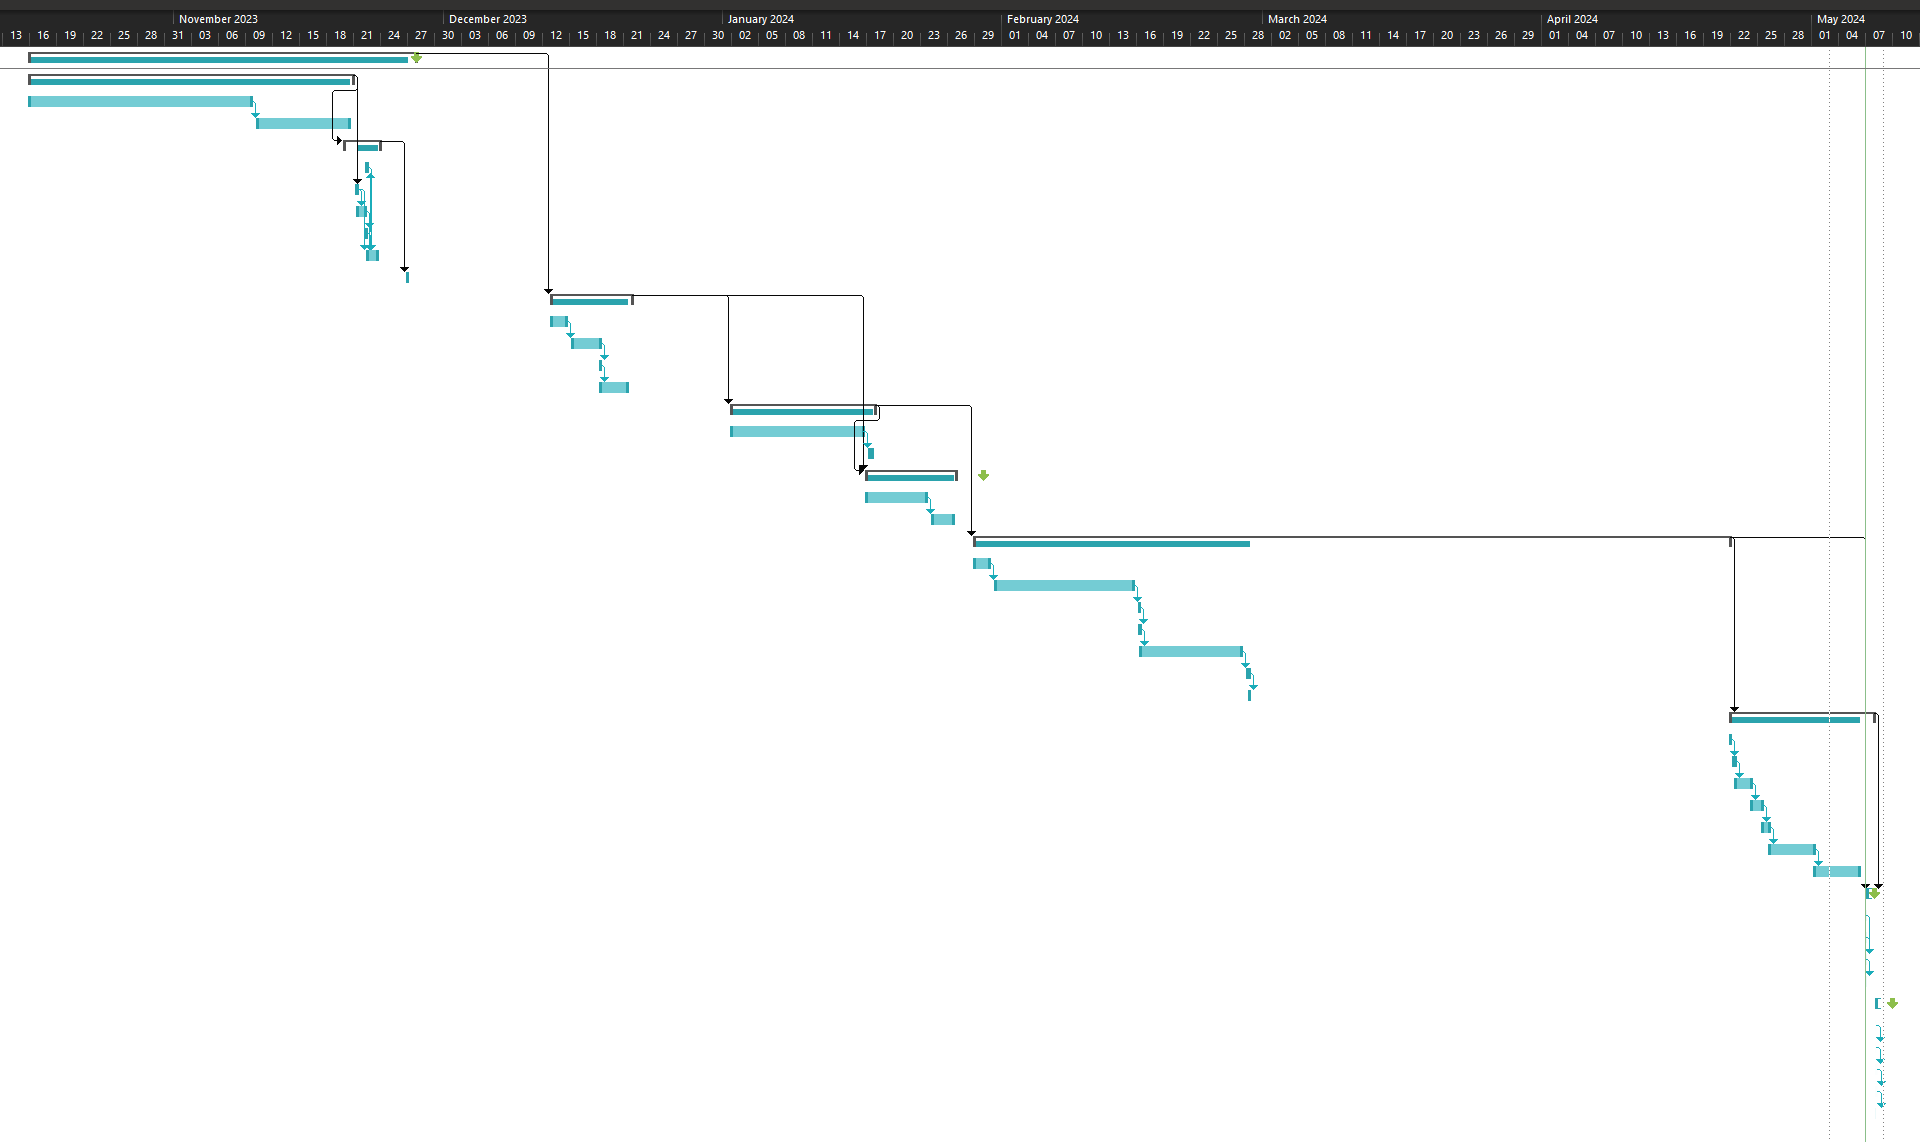
\includegraphics[clip, width=0.5\textheight]{Figures/GanttChart.png}
    \end{subfigure}
\end{figure}

% TODO: Performance - time taken before and after.
% TODO: Any peer review comments.
% TODO: Show manual testing.
